%%%%%%%%%%%%%%%%%%%%%%%%%%%%%%%%%%%%%%%%%
%
% Authors:
% Class by Felipe Portales-Oliva (f.portales.oliva@gmail.com) with template 
% content and modifications by Vel (vel@LaTeXTemplates.com)
%
% Enhanced by magicwenli 
%
%%%%%%%%%%%%%%%%%%%%%%%%%%%%%%%%%%%%%%%%%

\documentclass[
	12pt, % Default font size, values between 10pt-12pt are allowed
	cn,%letterpaper, % Uncomment for US letter paper size
	%cn, % Uncomment for Chinese
	%spanish, % Uncomment for Spanish
]{mwhw}

% Chinese and Fonts
\usepackage{ctex}

% Norm enhanced. Use \norm{}
\newcommand{\norm}[1]{\left\lVert#1\right\rVert}

% Template-specific packages
\usepackage[utf8]{inputenc} % Required for inputting international characters
\usepackage[T1]{fontenc} % Output font encoding for international characters
\usepackage{mathpazo} % Use the Palatino font

\usepackage{graphicx} % Required for including images

\usepackage{booktabs} % Required for better horizontal rules in tables

\usepackage{listings} % Required for insertion of code

\usepackage{enumerate} % To modify the enumerate environment

%----------------------------------------------------------------------------------------
%	ASSIGNMENT INFORMATION
%----------------------------------------------------------------------------------------

\title{Homework \#1} % Assignment title

\author{magicwenli} % Student name

\date{2020/4/13} % Due date

\institute{Xi'an Jiao Tong University \\ Department of Computer Science and Technology} % Institute or school name

\class{优化方法} % Course or class name

\professor{Mr. WenLi} % Professor or teacher in charge of the assignment

\IDnumber{21xxxxx}

%----------------------------------------------------------------------------------------

\begin{document}

\maketitle % Output the assignment title, created automatically using the information in the custom commands above

%----------------------------------------------------------------------------------------
%	ASSIGNMENT CONTENT
%----------------------------------------------------------------------------------------

\section*{问题 1}

\begin{problem}
	证明:范数$\norm{\cdot}$的对偶范数满足范数的定义
	\begin{equation*}
	    \norm{z}_*=sup\{z^Tx:\ \norm{x}\leq1\}=sup\{z^Tx:\ \norm{x}=1\}
	\end{equation*}
\end{problem}


%------------------------------------------------

\subsection*{解}
    \begin{equation*}
        \norm{z}_*=\max_{\norm{x}\leq 1}\sum{z_ix_i}
    \end{equation*}
    \begin{enumerate}
    \item 正定性:
    如果$z=0$,显然$\norm{0}_*=0$.
    \item 非负性:
    如果$z\neq 0$,则$\norm{x}\neq 0$. 由于$x=\frac{z}{\norm{z}}$,有$\norm{z}_*\leq \frac{\norm{z}^2_2}{\norm{z}}>0$.\\
    特别的,如果$\norm{z}_*=0$,则必有$z=0$.
    \item 齐次性:\\
    由范数定义,有:
    \begin{equation*}
        \norm{tz}_*=\max_{\norm{x}\leq 1} | z^Ttx|=\max_{\norm{x}\leq 1}|t||z^Tx |=|t| \max_{\norm{x}\leq 1} | z^Tx |=|t|\norm{z}_*
    \end{equation*}
    \item 满足三角不等式:\\
    unknow.
    
\end{enumerate}


%----------------------------------------------------------------------------------------



\end{document}


% \begin{center}
% 	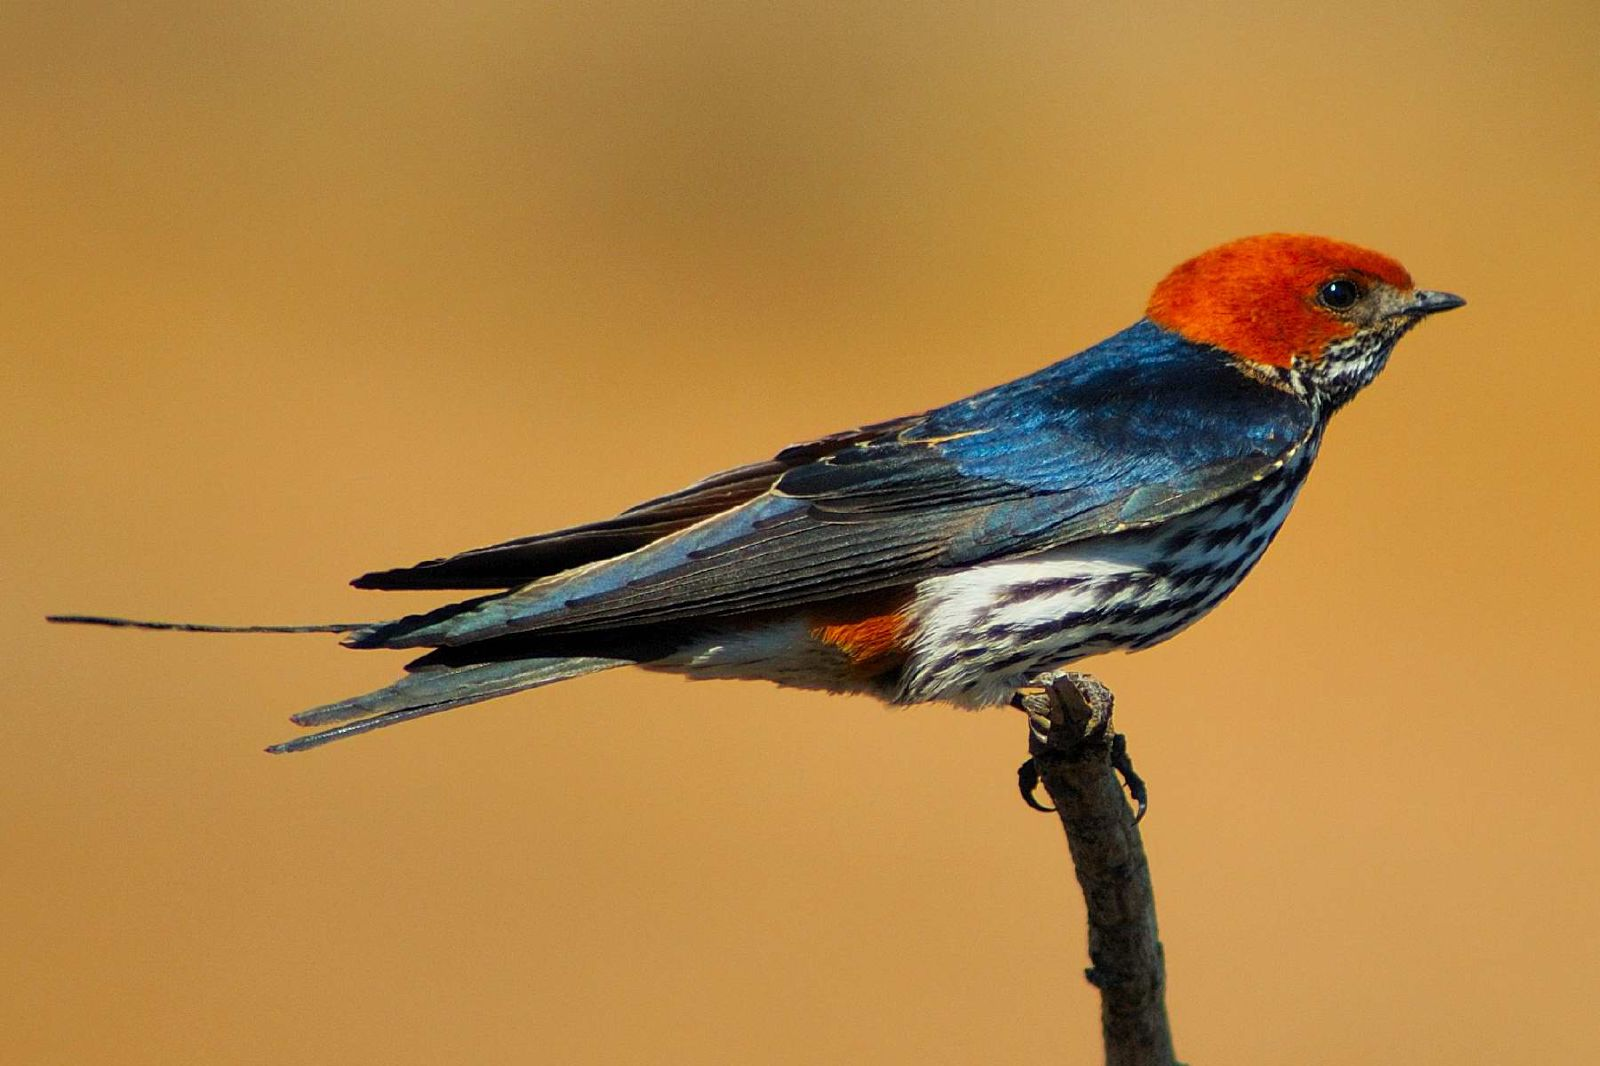
\includegraphics[width=0.5\columnwidth]{swallow.jpg} % Example image
% \end{center}
